%
% spline.tex
%
% (c) 2020 Prof Dr Andreas Müller, Hochschule Rapperswil
%

\section{Spline-Interpolation
\label{buch:section:spline}}
Die Hermite-Interpolation ermöglicht Aporoximationspolynome zu finden,
die sowohl Funktionswerte als auch Ableitungen an den Stützstellen mit
der zu approximierenden Funktion gemeinsam haben.
Dadurch wird der Fehler der Approximationspolynome zwar kleiner, aber
es entsteht das zusätzliche Problem, dass die Ableitungen der
Funktion bestimmt werden müssen.

Die Spline-Interpolation umgeht dieses Problem, indem sie an den
Stützstellen nicht die gleichen Steigungen verlangt, sondern Steigungen,
die zu einem möglichst ``wenig gekrümmten'' Graphen des Approximationspolynoms,
welches natürlich immer noch in den Stützstellen die vorgegebenen Werte
annehmen soll.
Die Steigungen in den Stützstellen sind also Lösungen eines
Optimierungsproblems, welches nicht die am besten passende, sonder
die ``schönste'' Kurve durch die Stützstellen sucht.

%
% Anforderungen an die Interplierende Funktion
%
\subsection{Anforderungen and die interpolierende Funktion
\label{buch:subsection:anforderungen}}
Gegeben seien wie früher Punkte
\[
a=x_0< x_1 < x_2< \dots < x_{n-1} < x_n = b
\]
auf und Funktionswerte $f_i$ einer im übrigen unbekannten, aber 
ausreichend glatten Funktion $f\colon [a,b]\to\mathbb R:x\mapsto f(x)$,
es ist also $f(x_i)=f_i$.

Gesucht ist eine stetige Funktion $g\colon[a,b]\to\mathbb R:x\mapsto g(x)$,
die die folgenden natürliche Eigenschaften haben soll:
\begin{enumerate}
\item
Die Funktion $g$ nimmt in allen Stützstellen die Werte der Funktion
$f$ an, es ist also $g(x_i)=f_i\;\forall 0\le i\le n$.
\item
Die Funktion $g$ ist stetig differenzierbar im ganze Interval.
Insbesondere existiert die Ableitung $g'(x)$ in jedem Punkt $x$ des
Intervals $[a,b]$, der Graph von $g$ kann also keine ``Knicke'' haben.
\item
Im inneren jedes Teilintervalles $[x_i,x_{i+1}]$ ist die Funktion $g$
beliebig oft stetig differenzierbar und die einseitigen Grenzwerte 
an den Enden der Teilintervalle existieren:
\[
\exists\; \lim_{x\to x_i+} g^{(k)}(x) \quad\forall 0\le i < n
\qquad\text{und}\qquad
\exists\; \lim_{x\to x_i-} g^{(k)}(x) \quad\forall 0< i \le n.
\]
Es wird nicht verlangt, dass die rechts- und linksseitigen Grenzwerte
an den inneren Stützstellen $x1,\dots,x_{n-1}$ übereinstimmen müssen.
\item
Der Graph von $g$ soll möglichst wenige gekrümmt sein.
Da die zweite Ableitung einer Funktion ein Mass für die Krümmung des 
Graphen ist, kann dieses Kriterium dadurch realisiert werdenn, dass
die Funktion $g$ unter allen Funktionen, die die Bedingungen 1--3 erfüllen,
das Integral
\[
J(g)
=
\int_a^b (g''(x) )^2\,dx
\]
minimiert.
\end{enumerate}

Man beachte, dass nirgends verlangt wird, dass die Ableitungen von $g$
an den Stützstellen irgendwie mit der Funktion $f$ in Verbingung steht.

%
% Das Optimierungsproblem
%
\subsection{Das Optimierungsproblem
\label{buch:subsection:variation}}
Zunächst ist nicht klar, ob das eben gestellt Optimierungsproblem überhaupt
eine Lösung hat. 
In jedem Teilinterval $[x_i,x_{i+1}]$ geht es um ein Problem der
folgenden Art.
Gesucht ist eine Funktion, die an den Intervallenden die vorgegebene
Werte $g(x_i)=f_i$ und $g(x_{i+1})=f_{i+1}$ annimmt, im Inneren des
Intervals beliebig oft stetig differenzierbar ist und zudem einen
Integralausdruck
\[
\int_{x_i}^{x_{i+1}} (g''(x))^2\,dx
\]
minimiert.

Diese Art von Problemen hat bereits Leonhard Euler in recht allgemeiner
Form untersucht und zu diesem Zweck das Gebiet der Variationsrechnung
geschaffen.
Sie tauchen in der Physik zum Beispiel in der folgenden Form auf.

\begin{beispiel}
Ein Teilchen der Masse $m$ bewegt sich entlang der $y$-Achse.
Zur Zeit $a$ befindet es sich bei $f_0$, zur Zeit $b$ bei $f_n$.
Auf das Teilchen wirkt ausserdem eine Kraft, die durch ihr Potential $V(y)$
beschrieben werden kann.
Die Geschwindigkeit zur Zeit $t$ ist $\dot y(t)$.
Die Differenz von kinetischer und potentieller Energie ist
die sogenannte Lagrange-Funktion
\begin{equation}
L(t,y,\dot{y})
=
\frac12m\dot{y}(t)^2
-
V(y(t)).
\label{buch:equation:mechlagrange}
\end{equation}
In der Physik wird gezeigt, dass die Bewegung des Teilchens durch diejenige
Funktion $y(t)$ beschrieben wird, welche das Integral
\[
\int_a^b L(t,y(t),\dot{y}(t))\,dt
\]
minimiert.
\end{beispiel}

\subsubsection{Die Euler-Lagrange-Gleichungen}
Um zu zeigen, dass die Interpolationsfunktion $g$ existiert, lösen
wir daher das folgende, wesentlich allgemeinere Problem.

\begin{satz}
\label{buch:satz:eulerlagrange}
Sei $L(x,y,y_1)$ eine in allen Argumenten beliebig oft stetig differenzierbare
Funktion auf $[a,b]\times \mathbb R \times \mathbb R$.
Es gibt eine glatte Funktion $y(x)$, die in den Intervalenden vorgegebene
Werte $y(a)=y_a$ und $y(b)=y_b$ annimmt und ausserdem das Integral
\[
J(y)
=
\int_a^b L(x, y(x), y'(x) ) \,dx
\]
minimiert,
sie ist Lösung der {\em Euler-Lagrange-Differentialgleichung}
\index{Euler-Lagrange-Differentialgleichung}
\begin{equation}
\frac{d}{dx} \frac{\partial L}{\partial y_1} (x,y(x),y'(x))
-
\frac{\partial L}{\partial y} (x,y(x),y'(x))
=
0.
\label{buch:variation:eulerlagrange}
\end{equation}
\end{satz}

\subsubsection{Richtungsableitung}
Die Verbindung zwischen den Extrema von $J(y)$ und der
Euler-Lagrange-Differentialgleichung entsteht durch die Ableitung 
von $J(y)$ nach $y$.
Zunächst ist allerdings zu klären, was diese Ableitung überhaupt bedeuten
soll.
Diese Ableitung soll in linearer Näherung wiedergeben können, was
passiert, wenn die Funktion $y(x)$ verändert wird.
Es gibt natürlich unendlich viele Stellen, in denen die Funktion
modifiziert werden kann, es handelt sich also um einen Ableitungsbegriff
in einem unendlichdimensionalen Vektorraum.
Die geometrische Intuition, die für den Begriff des Gradienten
verwendet wird, kann in der unendlichdimensionalen Situation versahgen,
wir müssen also etwas vorsichtiger sein.

Ungefährlich ist, die Veränderng von $J(y)$ nur in einer Richtung 
zu untersuchen.
Dazu ersetzen wir $y(x)$ durch $y_{\varepsilon}(x)=y(x)+\varepsilon h(x)$
und planen, den Parameter $\varepsilon$ zu verändern.
Es ist natürlich $y(x)=y_0(x)$.
Damit $y_{\varepsilon}(x)$ immer noch ein möglicher Kandidat für das Minimum
von $J(y)$ ist, müssen die Endpunkte von $y_{\varepsilon}(x)$ gleich sein,
es muss also
\begin{equation}
\left.
\begin{aligned}
y_{\varepsilon}(a)&=y(a) \\
y_{\varepsilon}(b)&=y(b) 
\end{aligned}
\right\}
\qquad\Rightarrow\qquad
h(a)=h(b)=0
\label{buch:variation:rand}
\end{equation}
gelten.

Die Funktion $J(\varepsilon) = J(y+\varepsilon h) = J(y_{\varepsilon})$
hängt jetzt nur noch von einem Parameter ab, die Ableitung davon ist
wohldefiniert.
Ist ausserdem $y$ ein Minimum, dann muss die Ableitung von
$J(y_{\varepsilon})$ nach $\varepsilon$ für $\varepsilon=0$
verschwinden, also
\[
0
=
\frac{d}{d\varepsilon} J(\varepsilon)\bigg|_{\varepsilon=0}
=
\frac{d}{d\varepsilon} J(y+\varepsilon h)\bigg|_{\varepsilon=0}.
\]
Dies muss für jede beliebige Funktion gelten, welche die Randbedingung
\eqref{buch:variation:rand} erfüllt.

\subsubsection{Integralprinzip}
Die Möglichkeit, die Funktion nur unter der minimalen Bedingung
\eqref{buch:variation:rand} frei zu wählen, schränkt die Funktion
$y(x)$ ein.
Dies ist der Inhalt des folgenden Prinzips
\begin{figure}
\centering
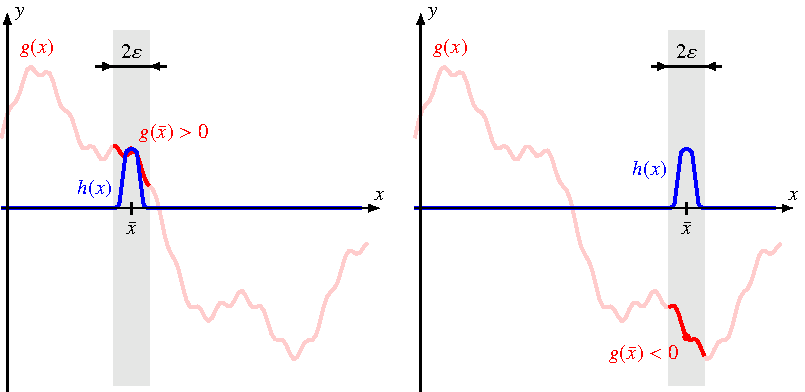
\includegraphics{chapters/30-interpolation/figures/integral.pdf}
\caption{Wenn das Integral von $g(x) h(x)$ für jede Funktion $h(x)$
verschwinden, dann muss auch $g(x)$ verschwinden.
In einer Umgebung eines Punktes $\bar{x}$, wo $g(\bar{x})\ne 0$ ist,
kann man $h(x)$ derart von $0$ verschieden wählen (blaue Kurve),
dass das Integral nicht verschwindet.
Der Widerspruch zeigt, dass $g(\bar{x})=0$ sein muss.
\label{buch:interpolation:figure:integralprinzip}}
\end{figure}

\begin{lemma}[Integralprinzip]
\label{buch:lemma:integralprinzip}
Sei $g(x)$ eine stetige Funktion auf dem Interval $[a,b]$.
Ausserdem gilt
\[
\int_a^b g(x)  h(x)\,dx = 0
\]
für jede auf $[a,b]$ definierte stetige Funktion mit $h(a)=h(b)=0$.
Dann ist $g(x)=0$.
\end{lemma}

\begin{proof}[Beweis]
Wir führen die Annahme, dass es einen Punkt $\bar{x}$ gibt mit
$g(\bar{x})\ne 0$, zu einem Widerspruch.

Nehmen wir also an, dass $g(\bar{x})>0$ ist.
Dann ist $g(x)>0$ wegen der Stetigkeit von $g$ auch noch ein einer
$\varepsilon$-Umgebung von $\bar{x}$ von $0$ verschieden.
Wir wählen $h(x)$ als stetige Funktion mit folgenden Eigenschaften
\begin{enumerate}
\item
Die Funktion wird nirgends negativ: $h(x)\ge 0$.
\item
$h(x)$ verschwindet ausserhalb der $\varepsilon$-Umgebung von $\bar{x}$.
\item
$h(\bar{x})=1$.
\end{enumerate}
Eine solche Funktion ist in
Abbildung~\ref{buch:interpolation:figure:integralprinzip} links
blau dargestellt.
Da $g(x)$ in der Umgebung $>0$ ist, folgt
\[
\int_a^b g(x)\,h(x)\,dx
=
\int_{\bar{x}-\varepsilon}^{\bar{x}+\varepsilon}
\underbrace{g(x)}_{\displaystyle>0}\,\underbrace{h(x)}_{\displaystyle\ge 0}\,dx
>
0,
\]
im Widerspruch zu den Voraussetzungen.

Der Fall $g(\bar{x})<0$ wird analog dazu behandelt, wie in
Abbildung~\ref{buch:interpolation:figure:integralprinzip} rechts
dargestellt.
\end{proof}

\subsubsection{Beweis von Satz~\ref{buch:satz:eulerlagrange}}
Wir gehen wie folgt vor: wir zeigen zunächst, dass eine solche Funktion
eine Differentialgleichung erfüllen muss.
Dann beziehen wir uns auf bekannte Sätze der Theorie der gewöhnlichen
Differentialgleichungen, die besagen, dass die Gleichung eine glatte 
Lösung hat.

Sei jetzt also $y(x)$ eine Funktion mit $y(a)=y_a$ und $y(b)=y_b$, die
das Integral $J(y)$ minimiert.
Ändern wir die Funktion ein klein wenig, dann muss der Wert von $J$ zunehmen.
Wir vollziehen die Änderung, indem wir eine Funktion $h(x)$
wählen mit $h(a)=0$ und $h(b)=0$.
Die Funktionen $y_\varepsilon= y+\varepsilon h$ erfüllen dann alle die
Bedingung $y_\varepsilon(a)=y_a$ und $y_\varepsilon(b)=y_b$, insbesondere
müssen sie alle einen Wert $J(g+\varepsilon h)$ ergeben, der grösser ist
als $J(g)$.
Insbesondere muss die Ableitung von $J(y+\varepsilon h)$ nach $\varepsilon$
an der Stelle $\varepsilon=0$ verschwinden.

Wir berechnen die Ableitung von $J(y+\varepsilon h)$ nach $\varepsilon$:
\begin{align}
0
=
\frac{d}{d\varepsilon} J(y+\varepsilon h)\bigg|_{\varepsilon=0}
&=
\frac{d}{d\varepsilon}
\int_a^b L(x, y(x) + \varepsilon h(x), y'(x)+\varepsilon h'(x))\,dx
\bigg|_{\varepsilon=0}
\notag
\\
&=
\int_a^b
\frac{\partial L}{\partial y}(x, y(x), y'(x)) \, h(x)
+
\frac{\partial L}{\partial y_1} L(x, y(x), y'(x) \, h'(x)
\,dx
\notag
\\
&=
\int_a^b
\frac{\partial L}{\partial y}(x, y(x), y'(x)) \, h(x)
\,dx
+
\int_a^b
\frac{\partial L}{\partial y_1} L(x, y(x), y'(x) \, h'(x)
\,dx
\label{buch:variation:zweiintegrale}
\end{align}
Das zweite Integral enthält die Ableitung $h'(x)$, über die wir nicht viel
wissen.
Wir können diese aber durch partielle Integration los werden:
\begin{align*}
\int_a^b
\frac{\partial L}{\partial y_1} L(x, y(x), y'(x) \, h'(x)
\,dx
&=
\biggl[\frac{\partial L}{\partial y_1}
L(x,y(x),y'(x))\,h(x)
\biggr]_a^b
-
\int_a^b \frac{d}{dx} \frac{\partial L}{\partial y_1}
L(x,y(x),y'(x))\,h(x) \,dx
\intertext{$h$ war so gewählt, dass die Werte, an den Intervalenden
verschwinden, also $h(a)=h(b)=0$.
Der erste Terme verschwindet daher und es bleibt}
&=
-
\int_a^b \frac{d}{dx} \frac{\partial L}{\partial y_1}
L(x,y(x),y'(x))\,h(x) \,dx.
\end{align*}
Einsetzen in \eqref{buch:variation:zweiintegrale} ergibt die Gleichung
\begin{equation}
0=
-
\int_a^b 
\biggl(
\frac{d}{dx}\frac{\partial L}{\partial y_1} (x,y(x), y'(x))
-
\frac{\partial L}{\partial y} (x,y(x),y'(x))
\biggr)
h(x)
\,dx.
\label{buch:variation:eulerintegralform}
\end{equation}

Gleichung \eqref{buch:variation:eulerintegralform}
muss für jede beliebige Funktion $h(x)$ gelten.
Wir möchten zeigen, dass das nur möglich ist, wenn die grosse Klammer
im Integral verschwindet.

Nehmen wir an, die grosse Klammer sei an einer Stelle im Intervall 
von $0$ verschieden.
Dann wird sie wegen der Stetigkeit auch in einer kleinen Umgebung dieser
Stelle immer noch das gleiche Vorzeichen haben.
Wir wählen eine Funktion $h$, die in der gleichen kleinen Umgebung
positiv ist und sonst überall verschwindet.
Das Integral muss dann nur noch über diese kleine Umgebung erstreckt
werden und die Funktion, die integriert wird, hat in der ganzen Umgebung
das gleiche Vorzeichen.
Insbesondere kann das Integral nicht verschwinden.
Somit ist gezeigt, dass die grosse Klammer verschwinden muss, oder dass
die Gleichung
\begin{equation}
\frac{d}{dx} \frac{\partial L}{\partial y_1} (x,y(x),y'(x)) 
-
\frac{\partial L}{\partial y}L(x,y(x),y'(x)).
\end{equation}
gelten muss.
Damit ist der Beweis von Satz~\ref{buch:satz:eulerlagrange} vollständig.

\begin{beispiel}
Wir wenden die Euler-Lagrange-Gleichung auf die Lagrange-Funktion
\eqref{buch:equation:mechlagrange} an, dabei erhalten wir
\[
\left.
\begin{aligned}
\frac{\partial L}{\partial y}
&=
-V'(y)
\\
\frac{\partial L}{\partial\dot{y}}
&=
m\dot{y}
\end{aligned}
\qquad\right\}
\quad\Rightarrow\quad
\frac{d}{dt} \frac{\partial L}{\partial \dot{y}} - \frac{\partial L}{\partial y}
=
\frac{d}{dt} 
m\dot{y} +V'(y)=0
\quad\Rightarrow\quad
m\ddot{y} = -V'(y).
\]
Dies ist das 2.~Newtonsche Gesetz.
\end{beispiel}

%
% Lösung des Optimierungsproblems
%
\subsection{Lösung des Optimierungsproblems
\label{buch:subsection:splineinterpolant}}
Leider lässt sich der Satz~\ref{buch:variation:eulerlagrange}
nicht direkt auf das Interpolationsproblem anwenden, weil im
Ausdruck $J(g)$ die zweite Ableitung von $g$ vorkommt.
Wir führen daher die Rechnung, die auf die Euler-Lagrange-Differentialgleichung
geführt hat, nochmals in diesem Spezialfall durch.
Wieder sei $h$ eine Funktion, die in jeder Stützstelle verschwindet.
Die Minimalitätsbedingung ist dann
\begin{align}
0
&=
\frac{d}{d\varepsilon}
\int_{x_i}^{x_{i+1}} (g''(x) + \varepsilon h''(x))^2 \,dx\bigg|_{\varepsilon=0}
\notag
\\
&=\int_{x_i}^{x_{i+1}} 2g''(x)h''(x) + 2\varepsilon h''(x)^2\,dx\bigg|_{\varepsilon=0}
\\
\notag
&=
\int_{x_i}^{x_{i+1}} 2g''(x) h''(x)\,dx.
\intertext{Wie bei der Euler-Lagrange-Gleichung können wir durch partielles
Integrieren die zweite Ableitung der Funktion $h$ los werden:}
0
&=
\biggl[ g''(x) h'(x) \biggr]_{x_i}^{x_{i+1}}
-
\int_{x_i}^{x_{i+1}} g'''(x) h'(x) \,dx
\notag
\\
&=
\biggl[ g''(x) h'(x) \biggr]_{x_i}^{x_{i+1}}
-
\biggl[ g'''(x) h(x) \biggr]_{x_i}^{x_{i+1}}
+
\int_{x_i}^{x_{i+1}} g^{(4)}(x) h(x)\,dx.
\label{buch:equation:splines:integiert}
\end{align}
Auf Grund der Definition von $h$ verschwindet der mittlere Term.

%
% Bedingungen im Inneren der Teilintervalle
%
\subsubsection{Bedingungen im Inneren der Teilintervalle}
Jetzt nutzen wir wieder die freie Wahlmöglichkeit der Funktion $h$
aus.
Wir können die Funktion so wählen, dass
$h(x_i)=h(x_{i+1})=h'(x_i)=h'(x_{i+1})=0$ ist, dann 
verschwinden die ersten beiden Terme.
Das Integral verschwindet nur dann immer, wenn der Integrand verschwindet,
wenn also $g^{(4)}(x)=0$ im Inneren jedes Teilintervals $[x_i,x_{i+1}]$.
Es folgt, dass in jedem Teilinterval die Funktion $g$ ein kubisches Polynom 
sein muss.

%
% Bedingungen an den Stützstellen
%
\subsubsection{Bedingungen an den Stützstellen}
Aus dem verbleibenden ersten Term von
Gleichung~\eqref{buch:equation:splines:integiert}
lässt sich noch mehr über die zweiten Ableitungen der Funktion $g$
schliessen.
Die Summe dieser Terme muss ja ebenfalls $0$ ergeben, also
\begin{align*}
0
&=
\sum_{i=0}^{n-1} 
\biggl[ g''(x) h'(x) \biggr]_{x_i}^{x_{i+1}}
=
\sum_{i=0}^{n-1}
\bigl( g''(x_{i+1}-) h'(x_{i+1}) - g''(x_i+) h'(x_i) \bigr)
\\
&=
-g''(x_0+)h'(x_0)
+
\sum_{i=1}^{n-1} h'(x_i) \bigl(g''(x_i-) - g''(x_i+)\bigr)
+
g''(x_n-)h'(x_n).
\end{align*}
Indem man für $h$ eine Funktion wählt, die an allen Stützstellen verschwindet
und in genau einer Stützstelle Ableitung $1$ hat, was mit einem
Hermite-Interpolationspolynom sicher möglich ist, schliesst man
\begin{equation}
g''(x_i-)=g''(x_i+)\quad\forall 1\le i< n.
\label{buch:equation:splineinner}
\end{equation}
Die Funktion ist also zweimal stetig differenzierbar.
Schliesslich müssen auch die Terme an den Enden der Summe verschwinden.
Eine Funktion $h$, die in allen Stützstellen zusammen mit der ersten
Ableitung in den inneren Stützstellen verschwindet und deren
erste Ableitung in genau einem der Endpunkte $1$ ist zeigt,
dass ausserdem
\begin{equation}
g''(x_0+) = g''(x_n-) = 0
\label{buch:equation:splinerand}
\end{equation}
sein muss.

%
% Ein Gleichungssystem für die Steigungen
%
\subsubsection{Ein Gleichungssystem für die Steigungen}
Zur Lösung des eingangs gestellten Interpolationsproblems ist jetzt
also für jedes Teilinterval $[x_i,x_{i+1}]$ ein kubisches Polynom $g_i(x)$
zu finden, mit folgenden Eigenschaften:
\begin{align*}
g_i(x_i)     &=f_i       &g_i(x_{i+1})  &=f_{i+1}   &0&\le i\le n &&\text{$2n+2$ Bedingungen}
\\
g_{i-1}'(x_i)&=g_i'(x_i) &g_{i-1}''(x_i)&=g_i''(x_i)&1&\le i< n &&\text{$2n$ Bedingungen}
\\
g_0''(x_0)   &=0         &g_n''(x_n)    &= 0        & &         &&\text{$2$ Bedingungen}
\end{align*}
Dies sind $4n+4$ lineare Bedingungen für $n+1$ Polynome, die je $4$
Koeffizienten haben.
Es sollte sich also ein lineares Gleichungssystem finden lassen, welches
diese Koeffizienten findet.

Aus Abschnitt~\ref{buch:section:hermite} ist bekannt, dass die kubischen
Polynome $g_i(x)$ durch die bereits bekannten Funktionswerte $f_i$
und die noch zu findenen Steigungen in den Stützstellen bestimmt sind.
Wir schreiben daher $s_i = g_i'(x_i)$ für die Steigungen und machen es
uns zum Ziel ein Gleichungssystem für die $s_i$ zu finden.

In Abschnitt~\ref{buch:subsection:hermite:zweistuetzstellen}
haben wir Hermite-Interopationspolynome für zwei Stützstellen
zusammengestellt.
Wir haben dort die Polynome $H_i$ und $H_i^1$ konstruiert, aus
denen sich mit der Substition $x\to (x-x_0)/m$ die
Hermite-Interpolationspolynome für das Interval $[x_0,x_0+m]$ 
bilden liess.
Wir bezeichnen die Länge des Intervalls $[x_i,x_{i+}]$
mit $m_i=x_{i+}-x_i$.

Die gesuchte Funktion im Interval ist daher
\begin{equation}
g_i(x) = f_i H_0((x-x_i)/m_i) + f_{i+1} H_1((x-x_i)/m_i)
+
s_i m_i H_0^1((x-x_i=)/m_i) + s_{i+1} m_i H_1^1((x-x_i)/m_i).
\label{buch:equation:spline:loesung}
\end{equation}
Diese Funktion hat die richtigen Funktionswerte und Ableitungen
an den Intervallenden.

Die Steigungen $s_i$ in \eqref{buch:equation:spline:loesung}
ist noch nicht bekannt, aber die Bedingung an die zweiten Ableitungen
wurde noch nicht ausgenutzt.
Die zweiten Ableitungen
\begin{align*}
i&=0
&
0
&=
g_0''(x_0)
=
-\frac{6f_0}{m_0^2} + \frac{6f_1}{m_0^2} -\frac{4s_0}{m_0} + \frac{2s_1}{m_0}
\\
i&=1
&
&\phantom{\mathstrut=\mathstrut}
g_0''(x_1)
=
\phantom{-}
\frac{6f_0}{m_0^2} -\frac{6f_1}{m_0^2} +\frac{2s_0}{m_0} -\frac{4s_1}{m_0}
\\
&
&
&=
g_1''(x_1)
=
-\frac{6f_1}{m_1^2}+\frac{6f_2}{m_1^2} - \frac{4s_1}{m_1}+\frac{2s_2}{m_1}
\\
i&=2
&
&\phantom{\mathstrut=\mathstrut}
g_1''(x_2)
=
\phantom{-}
\frac{6f_1}{m_1^2} -\frac{6f_2}{m_1^2} +\frac{2s_1}{m_1} -\frac{4s_2}{m_1}
\\
&
&
&=
g_2''(x_2)
=
-\frac{6f_2}{m_2^2}+\frac{6f_3}{m_2^2} - \frac{4s_2}{m_2}+\frac{2s_3}{m_2}
\\
&\qquad\vdots
&&
\\
i&=n
&
0&=
g_n''(x_n)
=
\phantom{-}
\frac{6f_{n-1}}{m_n^2}-\frac{6f_n}{m_n^2} +\frac{2s_{n-1}}{m_n}-\frac{4s_n}{m_n}
\end{align*}
In allen Gleichungen kommt der Faktor $2$ vor, den wir herausdividieren 
können.
Schaffen wir die Terme in $f_i$ auf die rechte Seite und sammeln die
Terme mit $s_i$ auf der linken Seite, erhalten wir das Gleichungssystem
\begin{equation}
\begin{linsys}{6}
\displaystyle\frac{2}{m_0} s_0
	&+&\displaystyle \frac{1}{m_0}s_1
		& &
			& &
				& &
				& &
					&=&\displaystyle3\frac{f_1-f_0}{m_0^2}
\\
\displaystyle \frac{1}{m_0} s_0
	&+&\displaystyle \biggl(\frac{2}{m_0}+\frac{2}{m_1}\biggr)s_1
		&+& \displaystyle \frac{1}{m_1}s_2
			& &
				& &
				& &
					&=&\displaystyle3\frac{f_2-f_1}{m_1^2}
\\
	& &\displaystyle\frac{1}{m_1} s_1
		&+&\displaystyle\biggl(\frac{2}{m_1}+\frac{2}{m_2}\biggr) s_2
			&+& \displaystyle\frac{1}{m_2} s_3
				& &
				& &
					&=&\displaystyle3\frac{f_3-f_2}{m_2^2}
\\
	& &
		& &
			& &
				&\ddots&
				&\ddots&
					& &\vdots\hspace*{10pt}
\\
	& &
		& &
			& &
			& &\displaystyle \frac{1}{m_{n-2}}s_{n-1}
				&+&\displaystyle \frac{2}{m_{n-1}}s_n
					&=&\displaystyle3\frac{f_n-f_{n-1}}{m_{n-1}^2}
\end{linsys}
\end{equation}
Die Koeffizientenmatrix und die rechte Seite dieses Gleichungsssytems sind
\[
A
=
\begin{pmatrix}
\displaystyle\frac{2}{m_0}
	&\displaystyle\frac{1}{m_0}
		&
			&
				&
					&
\\[8pt]
\displaystyle\frac{1}{m_0}
	&\displaystyle\frac{2}{m_0}+\frac{2}{m_1}
		&\displaystyle\frac{2}{m_1}
			&
				&
					&
\\[8pt]
	&\displaystyle\frac{1}{m_1}
		&\displaystyle\frac{2}{m_1}+\frac{2}{m_2}
			&\displaystyle\frac{1}{m_2}
				&
					&
\\[8pt]
	&
		&\displaystyle\frac{1}{m_2}
			&\ddots
				&\ddots
					&
\\[8pt]
	&
		&
			&\ddots
				&\ddots
					&\displaystyle\frac{1}{m_{n-2}}
\\[8pt]
	&
		&
			&
				&\displaystyle\frac{1}{m_{n-2}}
					&\displaystyle\frac{2}{m_{n-1}}
\end{pmatrix}
\qquad\text{und}\qquad
b
=
\begin{pmatrix}
\displaystyle3\frac{f_1-f_0}{m_0^2} \\[8pt]
\displaystyle3\frac{f_2-f_1}{m_1^2} \\[8pt]
\displaystyle3\frac{f_3-f_2}{m_2^2} \\[8pt]
\vdots \\[8pt]
\displaystyle3\frac{f_{n-1}-f_{n-2}}{m_{n-2}^2} \\[8pt]
\displaystyle3\frac{f_n-f_{n-1}}{m_{n-1}^2} 
\end{pmatrix}.
\]
Die Gleichungen werden besonders einfach, wenn alle Abstände gleich sind,
zum Beispiel $m=m_0=\dots m_{n-1}$.
Dann kann man die Gleichungen mit $m$ multiplizieren und bekommt für die
Koeffizientenmatrix und die rechte Seite
\[
A
=
\begin{pmatrix}
2&1& &      &      & \\
1&2&1&      &      & \\
 &1&2&1     &      & \\
 & &1&\ddots&\ddots& \\
 & & &\ddots&\ddots&1\\
 & & &      &     1&2
\end{pmatrix}
\qquad\text{und}\qquad
b
=
\frac{3}{m}
\begin{pmatrix}
f_1-f_0\\
f_2-f_1\\
f_3-f_2\\
\vdots\\
f_{n-1}-f_{n-2}\\
f_n-f_{n-1}

\end{pmatrix}
\]

%
% bezier.tex
%
% (c) 2020 Prof Dr Andreas Müller, Hochschule Rapperswil
%

\subsection{Bézier-Kurven und Splines in der Ebene
\label{buch:subsection:bezier}}
Spline-Interpolation kann auch verwendet werden um Kurven in der Ebene
oder im Raum zu approximieren.
In der Computergraphik ist dabei besonders wichtig, dass sich Kurvenpunkte
mit einfachen Operationen aus einer kleinen Zahl von Parametern berechnen
lassen, damit sie zum Beispiel von einem Graphikprozessor berechnet
werden können.
Dieser Abschnitt soll daher den Zusammenhang zwischen Bézier-Kurven und
Splines aufzeigen.


\subsubsection{Kurven in der Ebene}
Eine Kurve in der Ebene ist eine Abbildung
\[
\gamma \colon \mathbb R \to \mathbb R^2 : t \mapsto \gamma(t) = (x(t),y(t)),
\]
genannt die Parameterdarstellung der Kurve.
Man kann sich den Parameter $t$ als die Zeit vorstellen und die Funktionen
$x(t)$ bzw.~$y(t)$ als die Koordinaten eines sich auf der Kurve bewegenden
Punktes zur Zeit $t$.
Der Tangentialvektor
\[
\dot{\gamma}(t)
=
\frac{d\gamma(t)}{dt}
=
\begin{pmatrix}
\dot{x}(t)\\\dot{y}(t)
\end{pmatrix}
\]
kann entsprechend auch als der Geschwindigkeitsvektor zur Zeit $t$ 
intepretiert werden.

\begin{beispiel}
Ein Kreis in der Ebene kann beschreiben weren mit der Parameterisierung
\[
\gamma(t) = (\cos t, \sin t)
\qquad
\text{mit Geschwindigkeitsvektor}
\qquad
\dot{\gamma}(t)
=
\begin{pmatrix}
-\sin t\\\cos t
\end{pmatrix}.
\]
Der Betrag der Geschwindigkeit ist $|\dot{\gamma}(t)|^2=\sin^2t+\cos^2t=1$,
also konstant.
\end{beispiel}

\begin{beispiel}
Jeder Graph einer Funktion $f(x)$ kann als Kurve mit der Parameterisierung
\[
\gamma \colon \mathbb R\to\mathbb R^2 : t \mapsto (t, f(t))
\]
aufgefasst werden.
Der Tangentialvektor ist
\[
\dot{\gamma}(t)
=
\begin{pmatrix}
1\\f'(t)
\end{pmatrix}.
\]
Insbesondere ist die Geschwindigkeit $|\dot{\gamma}(t)|^2=1+f'(x)^2|>1$
im Allgemeinen nicht konstant.
\end{beispiel}

Das Beispiel zeigt, dass Graphen von Funktionen zwar als Kurven aufgefasst
werden können, als Bahnbeschreibung zum Beispiel für einen Roboter taugen
sie dagegen kaum.
Andererseits haben die Spline-Interpolationsfunktionen die schöne
Eigenschaft, dass die mittlere zweite Ableitung minimiert wird.
Sie sind daher ``die am wenigsten gekrümmten'' Kurven, die durch die
Stützstellen gehen. 
Eine solche Minimaleigenschaft für die Bahnkurve eines Roboters könnte eine
Bahn beschreiben, die sich mit maximaler Geschwindigkeit durchfahren lässt.
Die Zentripetalkraft, die die Räder in den Kurven aufbringen müssen,
kann nicht grösser sein als die Haftreibung.
Je grösser die Bahnkrümmung, desto grösser auch die Zentripetalkraft und
desto langsamer muss der Roboter durch die Kurve fahren, um nicht ins
Rutschen zu geraten.

Wir betrachten also eine Kurve, die durch die vorgegebene Punkte
\[
P_0 = (x_0, y_0),\;
P_1 = (x_1, y_1), \;
P_2 = (x_2, y_2),
\dots,
P_n=(x_n, y_n)
\]
gehen soll.
Wir fordern, dass der Punkt $P_i$ zum Zeitpunkt $t_i$ durchlaufen wird.
Wir entfernen uns hier etwas von der Anwendung einer Robotersteuerung,
da würde man nur die Punkte vorgeben und dann eine Bahn suchen, mit der
sich die Zeitpunkte $t_i$ so wählen lassen, dass die Gesamtzeit minimal
wird.
Die Funktionen $x(t)$ und $y(t)$ erfüllen jetzt also
\[
x(t_i) = x_i
\qquad\text{und}\qquad
y(t_i) = y_i.
\]
Das Problem, eine ebene Kurve durch die Punkte $P_i$ zu parametrisieren
ist jetzt also zerlegt worden in zwei unabhängige Interolationsprobleme
für die Funktionen $x(t)$ und $y(t)$.

Jedes in diesem Kapitel besprochene Interpolationsverfahren kann dafür
eine mögliche Lösung liefern, wobei sich die Spline-Interpolation wegen
der genannten Minimaleigenschaft besonders aufdrängt.
Dabei müssen zuerst die Steigungen und den Knotenstellen $t_i$ ermittelt
werden,
aus denen sich dann mittels Hérmite-Interpolation die Kurvenstücke
zwischen den Punkten $P_i$ als kubische Kurven berechnen lassen.
Die Steigungen in den Knotenstellen $t_i$ sind die Ableitungen
$\dot{x}(t_i)$ und $\dot{y}(t_i)$, d.~h.~es wir müssen zwischen
$P_i$ und $P_{i+1}$ eine kubische Kurve in der Ebene berechnen, die
Tangentialvektor $(\dot{x}(t_i),\dot{y}(t_i))^t$
bzw.~$(\dot{x}(t_{i+1}),\dot{y}(t_{i+1}))^t$ haben.
Eine besonders elegante Lösung für dieses Problem sind die Bézier-Kurven.

\subsubsection{Bézier-Kurven}
\begin{figure}
\centering
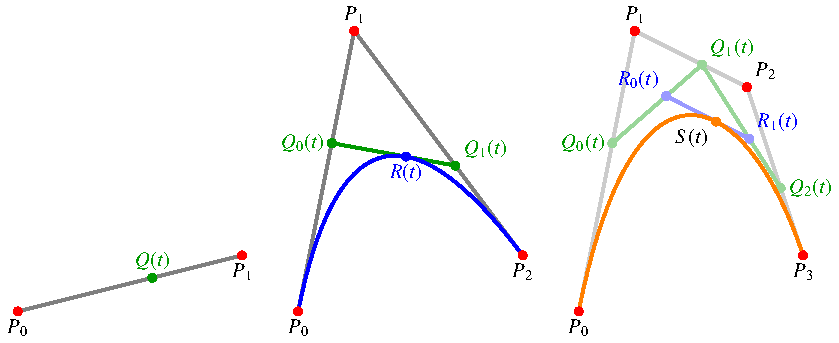
\includegraphics{chapters/30-interpolation/figures/bezier.pdf}
\caption{Bézier-Kurven bis zur Ordnung 3
\label{buch:interpolation:figure:bezier}}
\end{figure}
Die einfachste Verbindung zwischen zwei Punkten $P_0$ und $P_1$ mit
Ortsvektoren $p_0$ und $p_1$ ist eine Strecke, die man mit
\[
\gamma(t) = (1-t)p_0 + tp_1
\]
parametrisieren kann.
Der Tangentialvektor ist bereits bestimmt, er ist
\[
\dot{\gamma}(t) = -p_0 + p_1 = p_1-p_0.
\]
Die zwei Punkte legen den Tangentialvektor bereits fest, man kann
ihn nicht mehr frei wählen.

Kann man eine einfach zu berechnende Kurve finden, die den Punkt $P_0$
mit einem vorgegebenen Geschwindigkeitsvektor verlässt?
Paul de Casteljau hat vorgeschlagen, drei Punkte $P_0$, $P_1$ und $P_2$
zu verwenden und zunächst wie vorhin die Strecken 
\begin{align*}
q_0(t) &= (1-t) p_0 + t p_1 \\
q_1(t) &= (1-t) p_1 + t p_2 
\end{align*}
zu bilden.
Zur Zeit $t=0$ verlässt das erste Segment den Punkt $P_0$ mit der
Geschwindigkeit $p_1-p_0$.
Zur Zeit $t=1$ kommt das zweite Segment im Punkt $P_2$ an mit der
Geschwindigkeit $p_2-p_1$.
Man muss also zwischen $t=0$ und $t=1$ ``vom ersten Segment auf das zweite
wechseln''.
Dazu verbindet man die Punkte $q_0(t)$ und $q_1(t)$ mit einer Strecke und
wähle den Streckenparameter wieder als $t$.
Man erhält so eine Kurve
\begin{align*}
r(t)
&=
(1-t) q_0(t) + t q_1(t)
\\
&=
(1-t) \bigl( (1-t)p_0 + tp_1\bigr)
+
t \bigl( (1-t)p_1 + tp_2\bigr)
\\
&=
(1-t)^2 p_0 + 2t(1-t) p_1 + t^2 p_2.
\end{align*}
Der Geschwindigkeitsvektor zu den Zeiten $t=0$ und $t=1$ ist
\begin{align*}
\dot{r}(t)
&=
-2(1-t)p_0 + (2(1-t)-2t) p_1 + 2tp_2
\\
&=\begin{cases}
-2p_0+2p_1=2(p_1-p_0)&\qquad t=0
\\
-2p_1+2p_2=2(p_2-p_1)&\qquad t=1
\end{cases}
\end{align*}
Die gefundene Kurve verlässt also den Punkt $P_0$ genau in Richtung
auf $P_1$ und kommt im Punkt $P_2$ aus der Richtung von $P_1$ an.
Wir haben also eine quadratische Kurve gefunden, die einen Teil 
der Forderungen erfüllt.

Man nennt diese Kurve eine quadratische {\em Bézier-Kurve} mit
\index{Bézier-Kurve}
{\em Kontrollpunkten} $P_0$, $P_1$ und $P_2$.
\index{Kontrollpunkte}
Der Punkt $P_1$ kontrolliert die Start- und Ankunftsrichtung.

Die beiden Richtungen in Anfangs- und Endpunkten müssen unabhängig
voneinander vorgegeben werden können, wir versuchen daher, die
gleiche Konstruktion mit vier Kontrollpunkten durchzuführen.
Gegeben seien jetzt also die Punkte $P_0,\dots,P_3$.
Dann können wir drei Strecken
\begin{align*}
q_0(t) &= (1-t) p_0 + t p_1 \\
q_1(t) &= (1-t) p_1 + t p_2 \\
q_2(t) &= (1-t) p_2 + t p_3 
\end{align*}
konstruieren.
Die erste hat die ``richtige'' Startrichtung, die letzte die ``richtige''
Ankunfsrichtung.
Kombinieren wir $q_0(t)$ und $q_1(t)$, erhalten wir eine quadratische
Kurve, die vom Punkt $P_0$ mit der richtigen Geschwindigkeit weggeht,
die Kombination von $q_1(t)$ mit $q_2(t)$ liefert eine quadratische
Bézier-Kurve, welche im Punkt $P_3$ mit der richtigen Geschwindigkeit
ankommt.
Wir können also erneut kombinieren:
\begin{equation}
\left.
\begin{aligned}
r_0(t) &= (1-t)q_0(t) + t q_1(t) \\
       &= (1-t)^2 p_0 + 2t(1-t) p_1 + t^2 p_2
\\
r_1(t) &= (1-t)q_1(t) + t q_2(t) \\
       &= (1-t)^2 p_1 + 2t(1-t) p_2 + t^2 p_3
\end{aligned}
\quad
\right\}
\quad\Rightarrow\quad
s(t) = (1-t) r_0(t) + t r_1(t)
\end{equation}
Wir berechnen 
\begin{equation*}
\begin{linsys}{5}
s(t) &=& (1-t) \bigl( (1-t)^2 p_0 &+& 2t(1-t)         p_1 &+& t^2     p_2 &\bigr) & \phantom{\bigr)}\\
     & &                          & & t\bigl( (1-t)^2 p_1 &+& 2t(1-t) p_2 &+& t^2p_3\bigr) \\
     &=& (1-t)^3 p_0 &+& 3t(1-t)^2 p_1 &+& 3t^2(1-t) p_2 &+& t^3 p_3\rlap{.}\phantom{\bigr)}
\end{linsys}
\end{equation*}
Der Tagententialvektor an den Stellen $t=0$ und $t=1$ ist
\begin{align*}
\dot{s}(t)
&=
-3(1-t)^2p_0 + (3(1-t)^2-6t(1-t))p_1 + (6t(1-t)-3t^2)p_2 + 3t^2p_3
\\
\Rightarrow\qquad
\dot{s}(0) &= -3p_0+3p_1 = 3(p_1-p_0)
\\
\dot{s}(1) &= -3p_2 + 3p_3 = 3(p_3-p_2),
\end{align*}
die Kurve verlässt also wie erwartet den Punkt $P_0$ genau in Richtung 
auf $P_1$ und kommt genau aus der Richtung von $P_2$ in $P_3$ an.

Man kann auch die Spline-Funktionen wieder aus der zweidimensionalen
Kurve $s(t)$ rekonstruieren.
Gegeben sind dafür zwei Werte $y_0$ und $y_1$ und die Steigungen $m_0$ und
$m_1$ in den Punkten $x=0$ und $x=1$.
Der Graph des kubischen Polynoms $p(x)$ mit $p(0)=y_0$, $p(1)=y_1$,
$p'(0)=m_0$ und $p'(1)=m_1$ soll jetzt als Bézier-Kurve geschrieben werden.
Dazu müssen die Kontrollpunkte gefunden werden.
Es ist klar, dass $P_0=(0,y_0)$ und $P_3=(1,y_1)$.
Für die inneren Kontrollpunkte muss ein geeigneter $x$-Wert gewählt werden,
also
\[
P_1=
(x_1,y_0+x_1m_0)
\qquad
\text{und}
\qquad
P_2
=
(x_2,y_1-(1-x_2)m_1)
\]
Wählt man $x_1=\frac13$ und $x_2=\frac23$, dann wird
\begin{align*}
x(t)
&=
(1-t)^3\cdot 0 + 3t(1-t)^2\cdot \frac13 + 3t^2(1-t)\cdot \frac23 + t^3\cdot 1
\\
&=
t-2t^2+t^3 + 2t^2 -2t^3 + t^3 = t.
\end{align*}
Mit dieser Wahl ist also $x=t$, so dass das gesuchte Polynom $p(x)=y(x)$ wird:
\begin{align*}
p(x)
=
y(x)
&=
(1-x)^3 y_0
+
3x(1-x)^2\biggl(y_0+\frac13m_0\biggr)
+
3x^2(1-x) \biggl(y_1-\frac13m_1\biggr)
+
x^3 y_1
\\
&=
\bigl((1-x)^3+3x(1-x)^2\bigr)
y_0
+
x(1-x)^2 m_0
-
x^2(1-x) m_1
+
\bigl(3x^2(1-x)+x^3\bigr)
y_1
\\
&=
(1+2x)(1-x)^2 y_0
+
x(1-x)^2 m_0
+
x^2(x-1) m_1
+
x^2(3-2x) y_1.
\end{align*}
Die Koeffizienten von $y_0$, $y_1$, $m_0$ und $m_1$ sind die Polynome
\begin{equation}
\begin{aligned}
y_0:&&
H_0(x)
&=
2x^3-3x^2+1
&\quad&
&m_0:&&
H_0^1(x)
&=
x-2x^2+x^3
\\
y_1:&&
H_1(x)
&=
3x^2-2x^3
&\quad&
&m_1:&&
H_1^1(x)
&=
x^3-x^2
\end{aligned}
\label{buch:bezier:eqn:H}
\end{equation}
Die Polynome \eqref{buch:bezier:eqn:H} stimmen mit den Polynomen überein,
die in \eqref{buch:equation:hermite:h} gefunden worden sind.




